\setupsectionbase
\section{Аналитическая часть}

	\par В данном разделе рассматривается задача воспроизведения потокового аудио.
	Происходит постановка задачи, описывается предметная область. 
	Рассматриваются прикладные протоколы передачи потоковых данных.
	Дается анализ существующих средств воспроизведения аудиоданных в операционной системе iOS.

\subsection{Анализ предметной области}
	\par Воспроизведение потоковых аудиоданных на мобильных устройствах зависит от 
	протоколов потоковой передачи данных, форматов хранения аудиоданных, их обработки,
	а также от программных интерфейсов, предоставляемых разработчикам. 
	
	Зачастую используемые решения могут быть не универсальными, 
	а их выбор продиктован спецификой области применения и поставленными задачами.
	Так при построении системы транслирования радиоэфиров в реальном времени, можно принебречь качеством (разрешением звука) записи,
	а для системы прослушивания аудикниг, в которых важна дикция и подача чтеца, задержка передачи данных не является важным критерием.

\subsection{Цифровое представления аудиоданных}

	\par Звук состоит из слышимых изменений давления воздуха. 
	Звукозаписывающие устройства преобразуют изменение давления воздуха в переменное напряжение. 
	Чтобы представить звук в цифровом виде, необходимо преобразовать это изменяющееся напряжение в ряд чисел, представляющих его амплитуду. 
	Этот процесс известен как аналого-цифровое преобразование или дискретизация звука. 
	Числа, выдаваемые аналого-цифровым преобразователем, в общем случае произвольны.

	\par Изменение давления воздуха и, следовательно, соответствующее напряжение, создаваемое микрофоном, является непрерывным в двух измерениях.
	То есть значения непрерывно изменяются, и они существуют в каждый момент времени.
	Однако цифровая система, такая как компьютер, не может напрямую представлять непрерывный сигнал.
	Вместо этого применяется ряд процессов для оцифровки звука:
	\begin{itemize}
		\item[---] Дискретизация --- преобразование сигнала в конечное множество дискретных моментов времени;
		\item[---] Разрешение звука --- количество используемых дискретных уровней амплитуды сигнала;
		\item[---] Квантирование --- округление значения сигнала к одному из конечных дискретных уровней амплитуды. Обычно выражается в битах, то есть как логарифм по основанию 2 фактического числа;
	\end{itemize} 
	В результате вышеприведённых преобразований волна из своей непрерывной формы переходит в дискретизированную.
	
	Ниже, на рисунке \ref{fig:func} представлена непрерывная формы волны:

	\begin{figure}[!h]
		\center{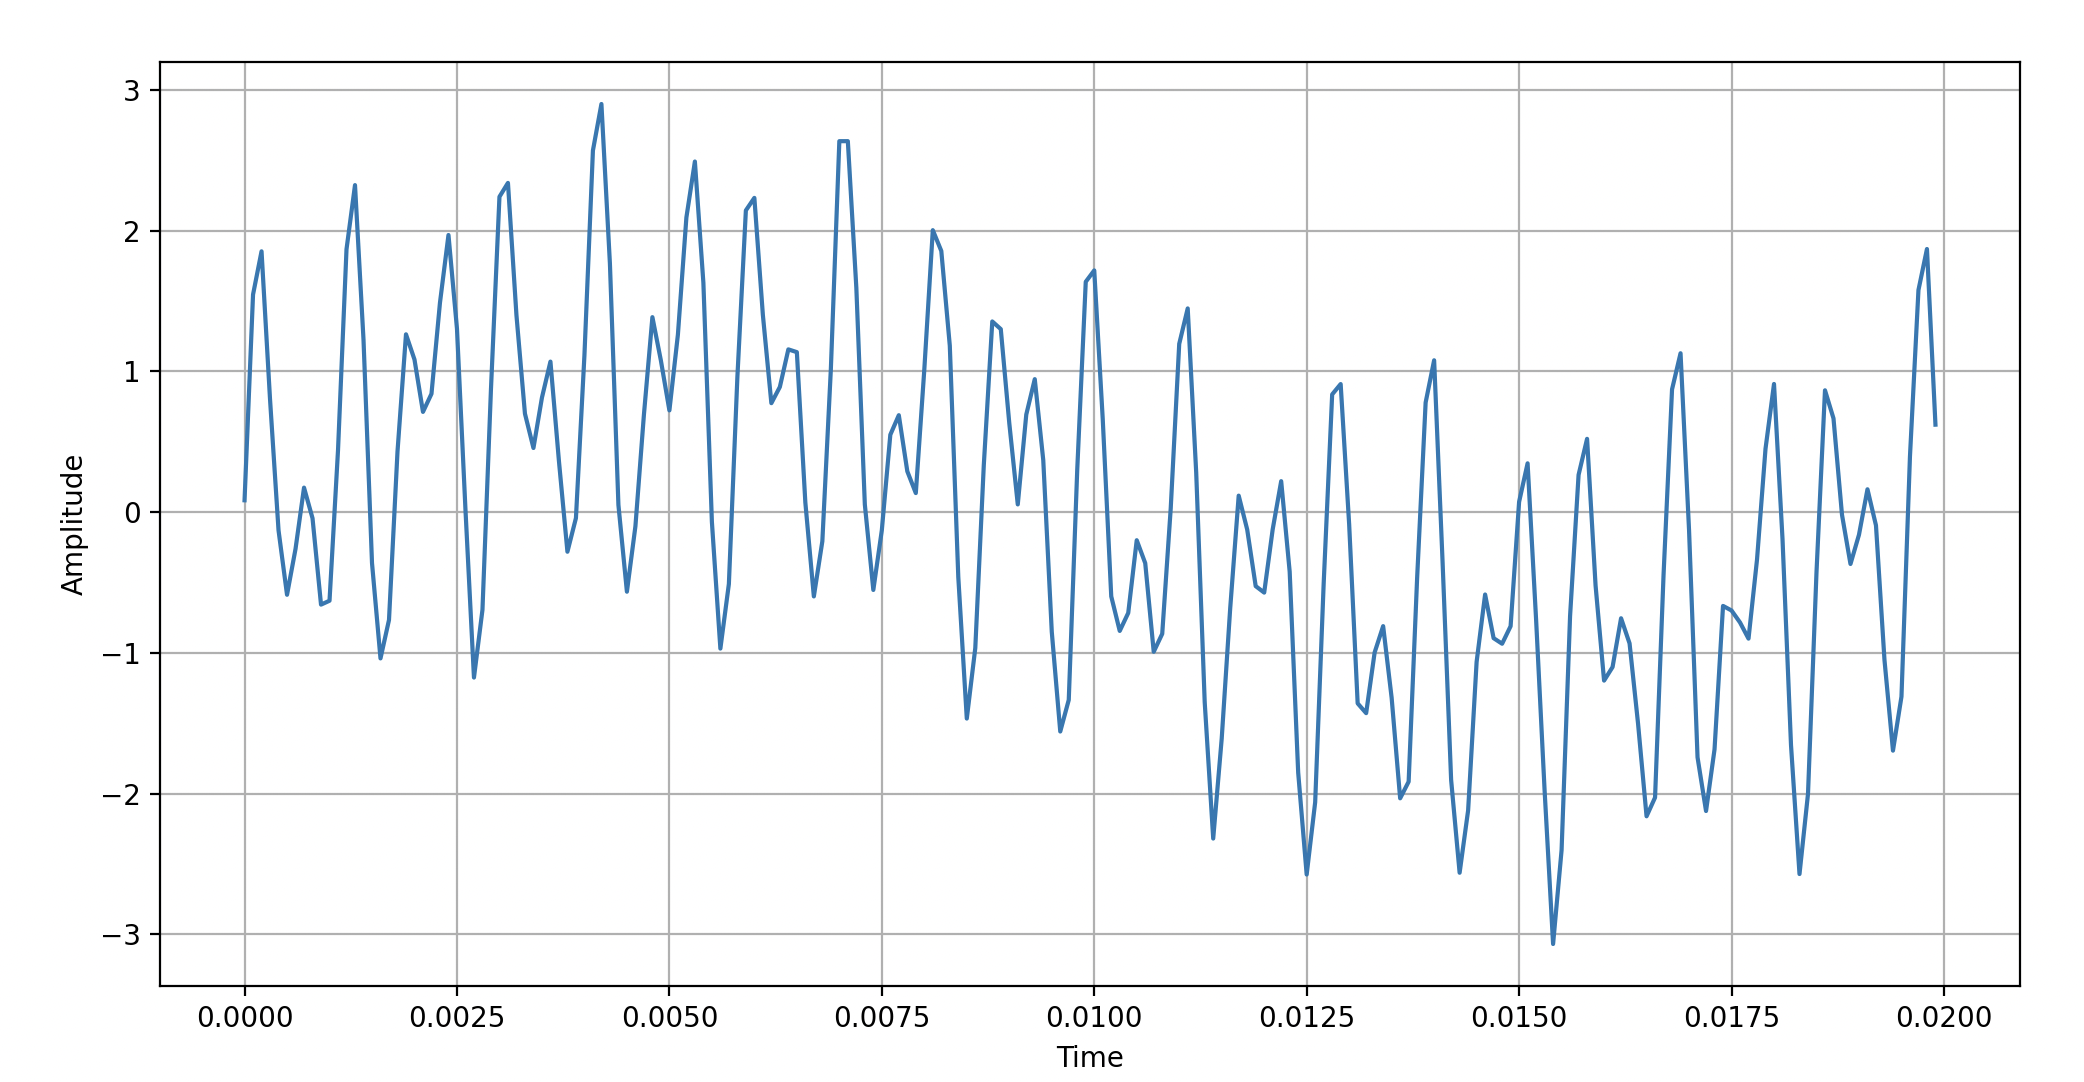
\includegraphics[scale=0.42]{img/func.png}}
		\caption{Непрерывная форма волны.}
		\label{fig:func}
	\end{figure}

	На рисунке \ref{fig:dfunc} представлено наложение дискретных уровней, полученных в ходе дискретизация, на непрерывную форму волны:

	\newpage
	\begin{figure}[!h]
		\center{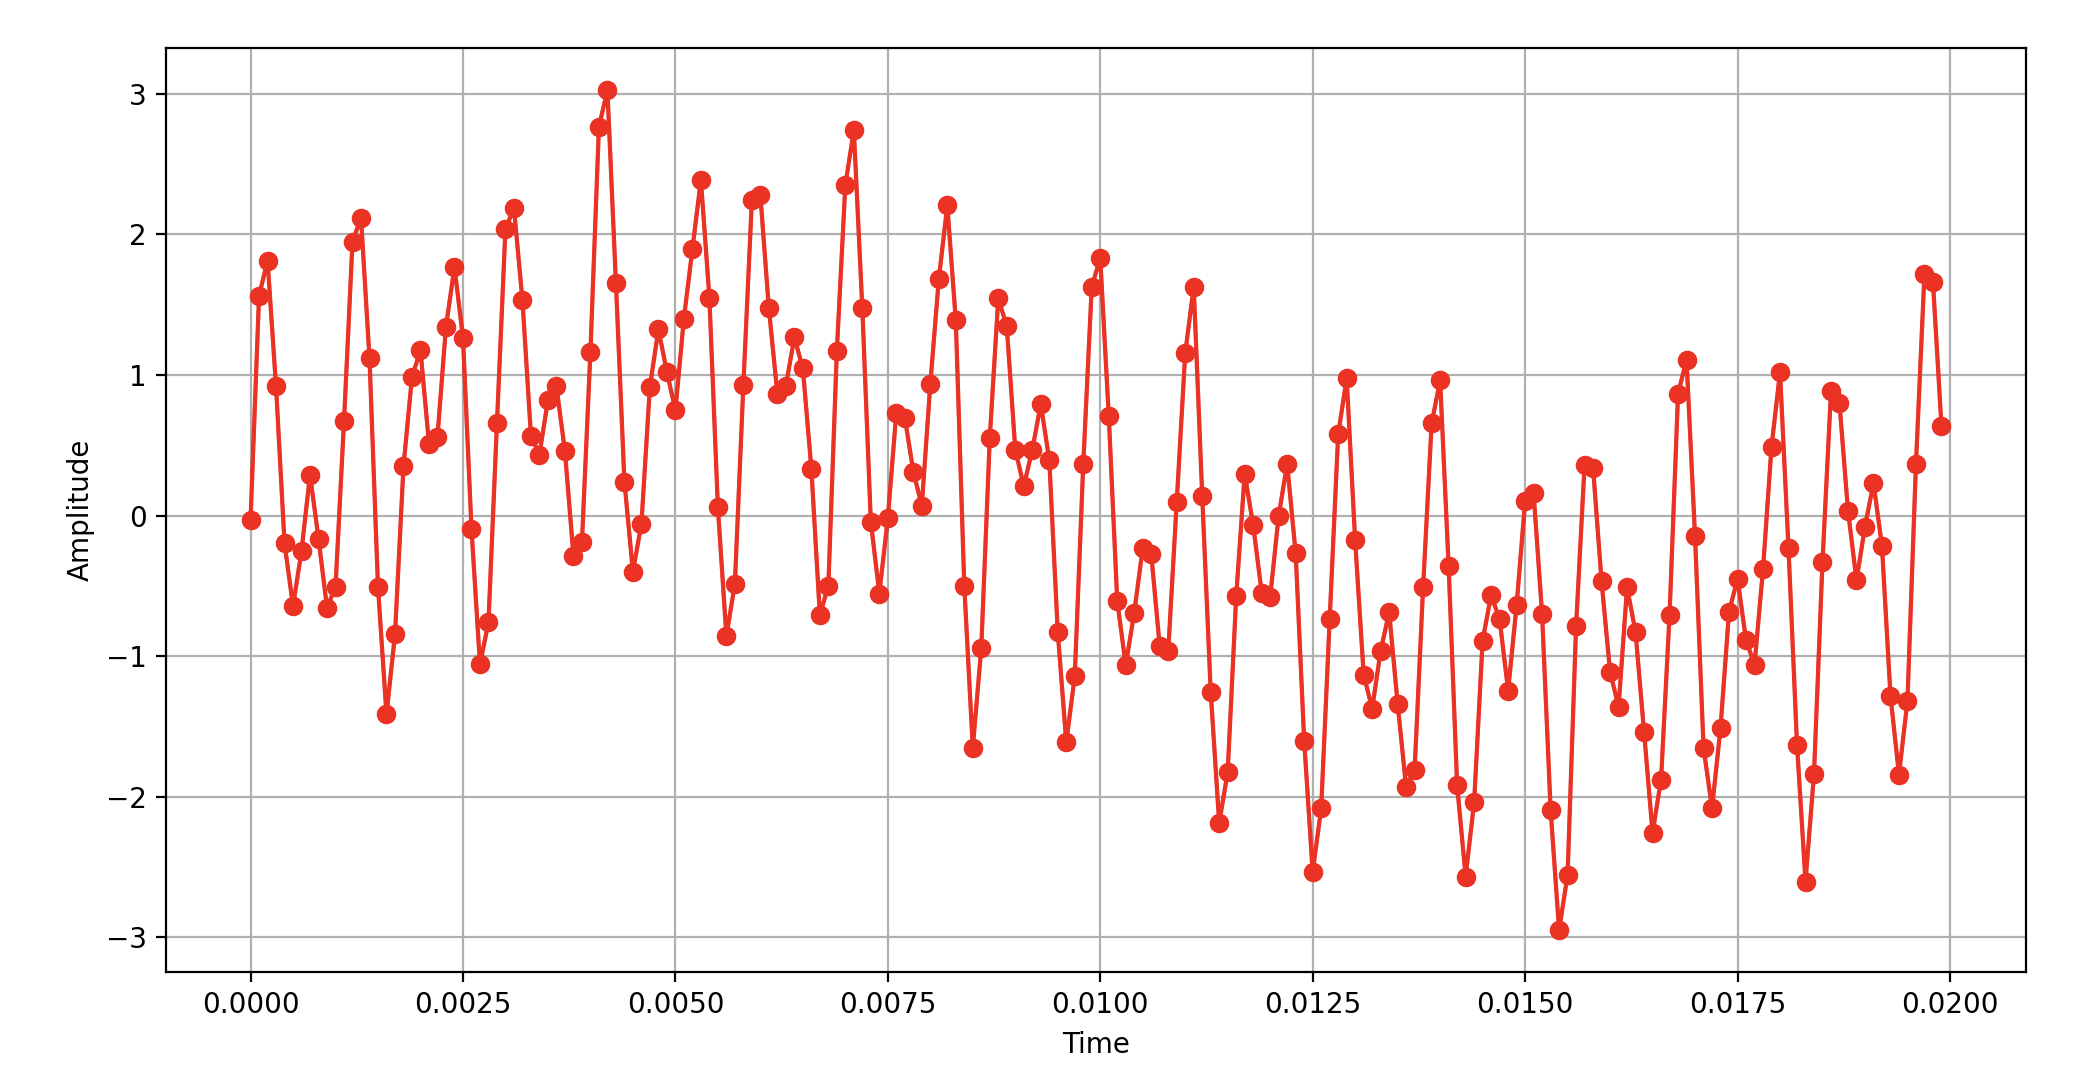
\includegraphics[scale=0.42]{img/dfunc.png}}
		\caption{Наложение дискретных уровней на непрерывную форму волны.}
		\label{fig:dfunc}
	\end{figure}

	\subsubsection*{Частота дискретизации}
	
		\par Частота дискретизации —-- это количество измерений амплитуды сигнала в секунду. Чем выше частота дискретизации, тем точнее дискретизированный сигнал будет представлять исходный сигнал. 

		\par Выбор частоты дискретизации определяется теоремой Котельникова о связи непрерывных и дискретных сигналов. 
		Эта теорема утверждает, что если максимальная частота, при которой исходный сигнал содержит энергию, равна $f_{c}$, 
		то, если он дискретизируется со скоростью, строго превышающей $2f_{c}$, 
		можно будет полностью восстановить исходный сигнал из дискретизированного сигнала, 
		то есть дискретизированный сигнал будет содержать всю информацию исходного сигнала.
		
		\par Другими словами, теорема Котельникова говорит о том, что непрерывный сигнал можно представить в виде интерполяционного ряда Фурье.
		Данное представление отображено в формуле \ref{eq:fur}:

		\begin{equation}\label{eq:fur}
			\begin{cases}
				x(t) = \sum\limits^{\infty}_{k = -\infty}x(k\Delta)sinc[\cfrac{\pi}{\Delta}(t - k\Delta)], \\
				0 < \Delta \leq \cfrac{1}{2f_{c}},
			\end{cases}
		\end{equation}
		где $\Delta$ -- интервал дискретизации (сек.).
	
\subsection{Анализ форматов хранения аудиоданных}

	\par В общем случае аудиофайлы могут быть не сжаты, а также не иметь явного формата.
	Чаще всего аудиоданные обрабатывают для хранения по специальному формату, хранят в файле специального формата,
	представляющим <<заголовок>>, а также тело --- выборку целых чисел, характеризующих цифровой сигнал для воспроизведения аудио.

	\par Заголовок может содержать:
	\begin{itemize}
		\item[---] тип файла;
		\item[---] разрешение звука;
		\item[---] частота дискретизации;
		\item[---] информацию о сжатие, если таковое имеется;
		\item[---] количество байтов, следующих за заголовком;
		\item[---] ​​информацию о название и исполнителе;
	\end{itemize} 

	\subsubsection{Необработанные звуковые файлы}
		\par Звуковые файлы, которые не имеют заголовка, а содержат только числовую выборку, характеризую цифровой сигнал, называются необработанными.
		Отсутствие явной информации о частоте дискретизации и разрешение позволяет использовать аудиоданные только по принятым соглашениям,
		которые принимаются между теми, кто упаковывает и использует данные аудио-файлы.

	\subsubsection{WAV (WAVE) формат}
		\par Для данного формата не применяется сжатие к битовому потоку, аудиозаписи хранятся с разными частотами дискретизации и битрейтами.  
		Однако WAV \cite{wave-audio} файлы имеют больший размер по сравнению с другими популярными форматами, такими как MP3, в которых используется сжатие с потерями для уменьшения размера файла при сохранении того же качества звука.
		Разрешение звука может быть как беззнаковым 8-битным, так и знаковым 16-битным (фрагменты дублируют информацию, найденную в других фрагментах). 
		Засчёт дубликатов блоков данных, характеризую цифровой сигнал в конкретный момент времени, обработка информации может занять дополнительное время.
		
		\par Заголовок файла содержит:
		\begin{itemize}
			\item[---] размер файла в байтах;
			\item[---] длину блока данных;
			\item[---] количество аудиоканалов;
			\item[---] битрейд;
			\item[---] частота дискретизации;
		\end{itemize}


	\subsubsection{MP4 формат}
		\par MP4 \cite{mp4} —-- это международный стандарт кодирования аудиовизуальных материалов, 
		из-за высокой степени сжатия, результирующие файлы имеют меньший размер с почти полным сохранением исходного качества.
		Данные в файле MP4 разделены на два раздела, первый из которых содержит мультимедийные данные, а второй содержит метаданные.
		Структуры в MP4 обычно называются атомами или блоками. Минимальный размер атома составляет 8 байт (первые 4 байта определяют размер, а следующие 4 байта определяют тип).

		\par Первый раздел содержит следующую информаию:
		\begin{itemize}
			\item[---] таблица выборок значений цифрового сигнала в момент времени;
			\item[---] заголовок аудиоданных, содержащий частоты дискретизаии (до 48 кГц) и разрешение звука;
			\item[---] количество аудиоканалов;
			\item[---] битрейд;
		\end{itemize}

		\par Второй раздел содержит следующую информаию:
		\begin{itemize}
			\item[---] дескриптор файла;
			\item[---] информацию о сжатие;
		\end{itemize}

	
	\subsubsection{MP3 формат}
		\par Файл MP3 \cite{mp3} состоит из фреймов, каждый из которых состоит из заголовка и блока данных. 
		Фреймы не являются независимыми и обычно не могут быть извлечены на произвольных границах переходов фреймов. 
		Блоки данных файла содержат информацию об аудио с точки зрения частот и амплитуд. 
		Заголовок идентифицирует начало допустимого кадра. 
		Затем следуют 3 бита, где первый бит показывает, что это стандарт MPEG, а оставшиеся 2 бита показывают, что используется уровень MPEG-1 Audio Layer \cite{mpeg}. 
		После этого значения будут различаться в зависимости от содержимого конкретного аудиофайла.

		\par Заголовок фрейма содержит следующую информацию:
		\begin{itemize}
			\item[---] информация о переходе на текщий фрейм;
			\item[---] идентификатор версии MPEG Audio;
			\item[---] описание фрейма;
			\item[---] бит, который показывает, что фрейм зашифрован;
			\item[---] битрейт;
			\item[---] частота дискретизации (от 8 кГц до 48 кГц);
			\item[---] приватный ключ шифрования;
		\end{itemize}
	
	\subsubsection{AAC формат}
		\par AAC (Advanced Audio Coding) \cite{acc} относится к стандарту цифрового кодирования звука, который представляет аудиофайлы на основе сжатия звука с потерями. 
		Он был запущен как преемник формата файла MP3 с учетом того, что у сторонних разработчиков возникли проблемы с реализацией новых идей в процессе кодирования, основанных на развитии методов сжатия данных. 
		AAC обеспечивает лучшее качество звука по сравнению с MP3 при той же скорости передачи данных. 
		Основные различия между AAC и MP3 с точки зрения улучшений заключаются в поддержке более широкого диапазона и частот дискретизации (от 8 кГц до 96 кГц).
		Разбиение по фреймам и содержание заголовка фрейма идентичны с MP3 форматом.
		
	\subsubsection{Сравнение форматов хранения аудиоданных}
		Сравнение рассмотренных форматов хранения аудиоданных рассмотрены в тблице \ref{tab:comparsion}. 
		Обозначения:
		\begin{itemize}
			\item[---] 1 --- поддержка частоты дискретизации более 48 кГц;
			\item[---] 2 --- наличие заголовка с метаинформацией;
			\item[---] 3 --- поддержка сжатия данных;
			\item[---] 4 --- фрагментаия данных цифрового сигнала;
		\end{itemize}
		\begin{table}[hbtp]
			\caption{Сравнение форматов хранения аудиоданных}
			\centering
			\label{tab:comparsion}
			% \resizebox{0.7\textwidth}{!}{%
			% \begin{tabular}{|l|l|l|l|l|}
			\begin{tabular}{|l|l|l|l|l|}
				\hline
				\textbf{Формат} & \textbf{1} & \textbf{2} & \textbf{3} & \textbf{4}   \\ \hline
				\text{WAV} & \textbf{+} & -          & -          &   -        \\ \hline
				\text{MP3} &   -        & \textbf{+} & \textbf{+} & \textbf{+} \\ \hline
				\text{MP4} &   -        & \textbf{+} & \textbf{+} & -          \\ \hline
				\text{ACC} & \textbf{+} & \textbf{+} & \textbf{+} & \textbf{+} \\ \hline
			\end{tabular}%
			% }
		\end{table}

		\par По результатам сравнения можно сделать вывод, что ниаболее оптимальными форматами хранения аудиоданных являются ACC и MP3.
		Принципиальное отличие заключается в диапазоне поддерживаемых частот дискретизации. 
		При требовании поддержки частоты дискретизации до 48 кГц форматы равноэффективны, но при необходимости в поддержке частоты до 96 кГц,
		необходимо использовать формат ACC.
		Стоит отметить, что формат WAV подходит в случае заранее принятных стандартов звукозаписи,
		при которых метаданные, хранящиеся в заголовках других форматов, будут известны. 

\subsection{Анализ протоколов передачи потоковых данных}

	\par Для передаче данных при стриминге необходимо использовать прикладные протоколы передачи данных,
	сжимающие данные для быстрой транспортировки, а также форматирующие данные в специальный формат.
	
	\subsubsection{HLS (HTTP Live Streaming)}

		\par На сегодняшний день HLS \cite{hls} является наиболее часто используемым протоколом для потоковой передачи. 
		Данный протокол создан на основе протокола прикладного уровня HTTP, использующий протокол транспортного уровня TCP \cite{tcp}.
		Концептуально HTTP Live Streaming состоит из трех частей:
		\begin{itemize}[leftmargin=1.6\parindent]
			\item[---] серверный компонент;
			\item[---] компонент доставки;
			\item[---] клиентское программное обеспечение.
		\end{itemize}

		\par В классической конфигурации аппаратный кодировщик принимает на вход аудио-файл. 
		Происходит кодировка аудио в ACС формат, 
		затем программный сегментатор разбивает поток на серии коротких медиафайлов, размещающихся на сервере. 
		Сегментатор создает и поддерживает файл-индекс, содержащий список медиафайлов. 
		Клиент считывает индекс, затем запрашивает перечисленные файлы по порядку и отображает их без остановок, разрывов между сегментами.
		На рисунке \ref{fig:hls} изображена схема принципа работы протокола HLS.

		\begin{figure}[!h]
			\center{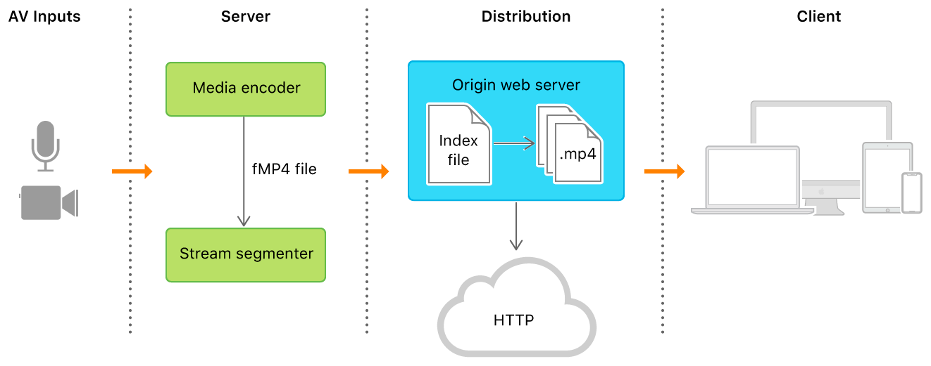
\includegraphics[scale=0.8]{img/hls.png}}
			\caption{Схема принципа работы протокола HLS.}
			\label{fig:hls}
		\end{figure}

		\par К достоинствам данного протокола можно отнести:
		\begin{itemize}[leftmargin=1.6\parindent]
			\item[---] сегментацая и индексация птока файлов, полученных в результате работы сегментатора;
			\item[---] поддержка ACC формата, что позволяет передавать аудиоданные с частотой дискретизации от 8 до 96 кГц;
			\item[---] гарантированная последовательная передачи пакетов без потерь;
		\end{itemize}

		\par К недостаткам данного протокола можно отнести:
		\begin{itemize}[leftmargin=1.6\parindent]
			\item[---] предворительная обработка исходного файла, которая заключается в разбиение и сжатие на подфайлы специального формата;
			\item[---] сильная задержка при передаче данных, которая не позволяет транслировать данные в режиме реального времени;
		\end{itemize}

	\subsubsection{Low-Latency HLS}

		\par Low-Latency HLS \cite{hls-ll} позволяет передавать медиа файлы на параллельных каналах, с помощью разделения медиафайлов на большее количество маленьких файлов CMAF Chunks. 
		Эти файлы называются частичными сегментами HLS. 
		Т.к. каждый частичный сегмент имеет меньшую длительность, он может быть упакован, передан или добавлен быстрее чем его родительский сегмент.
		Пока стандартный медиасегмент может быть длительностью 6 секунд каждый, частичный сегмент может быть до 1 секунды.

		\par Ускорение передачи данных достигается с помощью усложнения процесса предворительной обработки файла. 
		Происходит дробления подфайлов, полученных сегментатором, на частичные сегменты. 
		Создаётся список контекста сегментов, которые находятся в очереди на отправку данных.
		Параллельно происходит фильтрация списка, которая отбрасывает сегменты, которые считаются незначительными.

		\par По сравнения с стандартной организацией HLS, данный протокол обеспечивает более быструю передачу пакетов, 
		но требует дополнительной фильтрации сегментов, на которые делится исходный файл. 
		Также может происходить потеря какого-то блока данных цифрового сигнала, что приведёт к искажению воспроизведения аудиоданных.


	\subsubsection{RTSP (Real-Time Streaming Protocol)}

		\par RTSP \cite{rtsp} – протокол прикладного уровня. 
		Реализует потоковую прередачу медиа данных в реальном времени, а также устанавливает и управляет либо одним, либо несколькими синхронизированными во времени потоками.
		Источники данных могут быть как источниками реального времени, так и хранимыми.
		RTSP поддерживает как передачу данных, сегментируемых аппаратным сегментатором, так и передачу с помощью датаграм, благодаря чему совместим и с протоколом транспортного уровня TCP \cite{tcp}, и с UDP \cite{udp}.

		\par Механизм передачи данных в реальном времени обусловлен отсутствием предворительной фильтрации сегментов аудиофайлов. 
		Аналогово-цифровой преобразователь полностью перенаправляет поток данных на RTSP сервер, который сегментирует поступающие данные, 
		сжимает и конвертирует их в ACC или MP3 формат.

		\par К достоинствам данного протокола можно отнести:
		\begin{itemize}[leftmargin=1.6\parindent]
			\item[---] отсутствие предворительной обработки поступаемых данных;
			\item[---] передача данных в режиме реального времени с задержкой до 2 секунд;
			\item[---] гарантированная последовательная передачи пакетов;
		\end{itemize}

		\par К недостаткам данного протокола можно отнести:
		\begin{itemize}[leftmargin=1.6\parindent]
			\item[---] потеря пакетов данных при обработке аналогово-цифрового сигнала;
			\item[---] сжатие данных обусловливает частоту дискретизации до 48 кГц;
		\end{itemize}
	
	\subsubsection{Сравнение протоколов передачи потоковых данных}
		Сравнение рассмотренных протоколов передачи потоковых данных рассмотрены в тблице \ref{tab:stream-prot}. 
		Обозначения:
		\begin{itemize}
			\item[---] 1 --- поддержка частоты дискретизации более 48 кГц;
			\item[---] 2 --- трансляция в режиме реального времени;
			\item[---] 3 --- гарантированная последовательная передача пакетов без потерь;
			\item[---] 4 --- необходимость предварительной обработки аудиофайлов перед трансляцией; 
		\end{itemize}

		\newpage
		\begin{table}[hbtp]
			\caption{Сравнение протоколов передачи потоковых данных}
			\centering
			\label{tab:stream-prot}
			\begin{tabular}{|l|l|l|l|l|}
				\hline
				\textbf{Протокол} & \textbf{1} & \textbf{2} & \textbf{3} & \textbf{4}  \\ \hline
				\text{HLS}             & \textbf{+} & -          & \textbf{+} & \textbf{+} \\ \hline
				\text{Low-Latency HLS} & \textbf{+} & -          & -          & \textbf{+} \\ \hline
				\text{RTSP}            &   -        & \textbf{+} & -          & -          \\ \hline
			\end{tabular}%
			% }
		\end{table}

		\par По результатам сравнения можно сделать вывод, протоколы семейства HLS хорошо подходят для транслирования предварительно обработанных аудио-файлов с частотой дискретизации более 48 кГц, 
		но не поддерживают передачу данных в режиме реального времени. 
		Протокол RTSP, напротив, лучше подходит для трансляции в реальном времени, но плохо поддерживает файлы с большой частотой дискретизации.
		Стоит отметить, что при использовании Low-Latency HLS и RTSP возможна потеря данных при трансляции.

\subsection{Анализ существующих средств воспроизведения аудиоданных в операционной системе iOS}
	
	Воспроизведение аудиоданных зависит от программных компонентов, а также доступных ресурсов, предоставляемых разработчикам.
	Ниже рассмотрены доступные подходы и механизмы для воспроизведения аудио в операционной системе iOS \cite{iOSOS}.

	\subsubsection{Воспроизведение загруженных в оперативную паять аудиоданных}
		\par Один из подходов к воспроизведению аудиоданных в операционной системе iOS заключается в обработке и загрузке аудио-файла целиком в оперативную память устройства.
		Работа происходит с аудио-файлами целиком, в оперативную память устройства выгружаются заголовки и блоки данных цифрововго сигнала, 
		что напрямую связывает возможность проигрывания аудио с доступным размером оперативной памяти. 
		
		\par Программным компонентом который позволяет воспользоваться данным подходом является AVPlayer, позволяющий работать с локальными файлами устройства, имеющими форматы MP3, MP4, ACC.
		Поддержка частоты дискретизации вплоть до 96 кГц, а также разрешение звука до 32 бит даёт возможность воспроизведение и увправления
		аудиоданных выского качества.

		\par К плюсам данного подхода можно отнести:
		\begin{itemize}
			\item[---] поддержка аудио-файлов с частотой дискретизации до 96 кГц;
			\item[---] поддержка аудио-файлов с разрешеним звука до 32 бит;
			\item[---] отсутствие задержек, обословленных получением пакетов данных при потоковой передаче;
			\item[---] поддержка форматов ACC, MP3; 
		\end{itemize}

		\par К недостаткам данного подхода можно отнести:
		\begin{itemize}
			\item[---] полная выгрузка аудиоданных в оперативную память, отсутствие сегментации файла;
			\item[---] отсутствует поддержка потокового воспроизведение данных:
		\end{itemize}


	\subsubsection{Воспроизведение аудиоданных с помощью системного сегментатора}
		\par Системный сегментатор позволяет обрабатывать пакеты данных при потоковой передаче аудиоданных.
		Происходит обработка сегментов, сформированных протаколами потоковой передачи данных (HLS, RTSP),
		которая заключается в получении заголовка фрейма блока данных, который подаётся для воспроизведения.
		В операционной системе iOS сегментацию пакетов аудиоданных содержут два програмных компонента: AVAudioPlayer \cite{avplayer}, AVAudioEngine \cite{avengine}.
		
		\par AVAudioPlayer поддерживает протокол потоковой передачи данных HLS, частоту дискретизации до 48 кГц, а также разрешение звука до 16 бит.
		Основной особенностью является управление воспроизведением аудио.
		
		AVAudioEngine поддерживает протоколы HLS и RTSP, а также разрешение звука до 32 бит.
		Данных програмный компонент не предпологает управление воспроизведением аудиоданных, но даёт возможнось наложения эфектов аудиофильтров и работы с нотной матрицей.

	\subsubsection{Воспроизведение аудиоданных с помощью взаимодействия с звуковой картой}
		\par Работа с звуковой картой устройства поддерживается с помощью програмного интерфейса CoreAudio \cite{coreaudio},
		который поддерживает обработку пакетов аудиоданных для потокового воспроизведения, различные частоты дискретизации и разрешения звука, наложение звуковых эффектов,
		работу с нотной матрицей и обработку выделения памяти для хранения сегментов данных цифрового сигнала.
		При работе с аудиокартой необходимо реализовывать собственный сегментатор, так как системная поддержка стандартов протоколов потоковой передачи данных отсутствует.
		
		\par К плюсам данного подхода можно отнести:
		\begin{itemize}
			\item[---] поддержка аудио-файлов с различными частотами дискретизации;
			\item[---] поддержка аудио-файлов с различными разрешениями звука;
			\item[---] поддержка обработки пакетов аудиоданных для потокового воспроизведения; 
		\end{itemize}

		\par К недостаткам данного подхода можно отнести:
		\begin{itemize}
			\item[---] отсутствие поддержки системного сегментатора;
			\item[---] отсутствие поддержки форматов аудио-файлов, все звуковые файлы принимаются в качестве необработанных;
			\item[---] отсутствие поддержки обработки стандартов протоколов потоковой передачи данных;
		\end{itemize}
		

	\subsubsection{Сравнение средств воспроизведения аудиоданных в операционной системе iOS}
		Сравнение рассмотренных средств воспроизведения аудиоданных в операционной системе iOS рассмотрены в таблице \ref{tab:ios}. 
		Обозначения:
		\begin{itemize}
			\item[---] 1 --- поддержка частоты дискретизации более 48 кГц;
			\item[---] 2 --- поддержка воспроизведения потоковых данных;
			\item[---] 3 --- воспроизведение в режиме реального времени;
			\item[---] 4 --- наложение звуковых эффектов;
			\item[---] 5 --- наличие встроенного сегментатора для обработки потоковых данных;
			\item[---] 6 --- поддержка MP3 или ACC форматов ауди-файлов; 
		\end{itemize}

		\begin{table}[hbtp]
			\caption{Сравнение протоколов передачи потоковых данных}
			\centering
			\label{tab:ios}
			\begin{tabular}{|p{300pt}|l|l|l|l|l|l|}
				\hline
				\textbf{Подход} & \textbf{1} & \textbf{2} & \textbf{3} & \textbf{4} & \textbf{5} & \textbf{6}  \\ \hline
				Воспроизвведение загруженных в оперативную паять аудиоданных           & \textbf{+} & -          & -          & \textbf{+} & -          & \textbf{+} \\ \hline
				Воспроизведение аудиоданных с помощью системного сегментатора          & -          & \textbf{+} & \textbf{+} & -          & \textbf{+} & \textbf{+} \\ \hline
				Воспроизведение аудиоданных с помощью взаимодействия с звуковой картой & \textbf{+} & \textbf{+} & \textbf{+} & \textbf{+} & -          & -          \\ \hline
			\end{tabular}%
			% }
		\end{table}

		\par По результатам сравнения можно сделать вывод, что для воспроизведения потокового аудио подход с воспроизвведением загруженных в оперативную паять аудиоданных не подходит.
		Системный cегментатор позволяет обрабатывать пакеты потоковых аудиоданных, с использованием протоколов HLS и RTSP.
		Для воспроизведение аудио с частотой дискретизации более 48 кГц, то необходимо использовать программный компонет CoreAudio для взаимодействия с аудиокартой устройства.


\pagebreak


